\documentclass[12pt]{report}
%%%%% fonts %%%%%%%%%%%%%%%%%%%%%%%%%%%%%%%%%%%
\usepackage{fontspec}
\setmainfont{Charis SIL}
%%%%% graphics %%%%%%%%%%%%%%%%%%%%%%%%%%%%%%%%
\usepackage{graphicx}
\graphicspath{ {figures/}}
\usepackage{longtable}
%%%%% page setting %%%%%%%%%%%%%%%%%%%%%%%%%%%%
\usepackage[a4paper,width=150mm,top=25mm,bottom=25mm,bindingoffset=6mm]{geometry}
\usepackage{fancyhdr}
\pagestyle{fancy}
%%%%% Biblatex package %%%%%%%%%%%%%%%%%%%%%%%%
\usepackage[hidelinks]{hyperref}
\usepackage[backend=biber,style=unified,maxcitenames=3,maxbibnames=99,natbib=true]{biblatex}
%%%%% caption %%%%%%%%%%%%%%%%%%%%%%%%%%%%%%%%%
\usepackage{caption}
\usepackage{subcaption}
%%%%% Linguistics packages %%%%%%%%%%%%%%%%%%%%
\usepackage{tipa}
\renewcommand{\tipa}[1]{\textipa{#1}}
%%%%% Math package %%%%%%%%%%%%%%%%%%%%%%%%%%%%
\usepackage{mathtools}
\usepackage{amssymb}
\usepackage{urwchancal}
\usepackage{amsfonts}
%%%%%%%%%%%%%%%%%%%%%%%%%%%%%%%%%%%%%%%%%%%%%%%
\title{Positional Asymmetry of Consonants: A Preliminary Study}
\author{Cong Luan Tran}


\addbibresource{references.bib}
\begin{document}

\begin{titlepage}
    \begin{center}
        \vspace*{1cm}
        
        \Huge
        \textbf{Title}
            
        \vspace{0.5cm}
        \LARGE
        Subtitle
            
        \vspace{1.5cm}
            
        \textbf{Cong Luan Tran}
            
        \vfill
        \LARGE
        \textbf{BA thesis Linguistics}\\
        
        \vspace{0.5cm}
        
        \Large 
        Under the supervision of 
        
        \vspace{0.5cm}
        \LARGE
        \textbf{Paul Boersma}
        
        \vspace{0.8cm}
            
        %\includegraphics[width=0.4\textwidth]{}
            
        \Large
        Faculty of Humanities\\
        University of Amsterdam\\
        date 
        
        \vfill
    \end{center}
\begin{flushright}
Student number: 12530263
\end{flushright}
\end{titlepage}

\tableofcontents

\chapter{Introduction}
\section{Motivation}

\citet{wals-9} claimed that the velar nasal  /ŋ/ is exceptional in its phonotactic distribution: virtually all languages that have phonemic /ŋ/ allow it in the final position, while over one-third of those languages prohibit it in the initial position. In fact, of 20 chapters concerning phonology in \citet{wals}, \citeauthor{wals-9}'s The Velar Nasal is the only chapter that deals with only a single segment. This creates an impression that the distributional asymmetry of /ŋ/ is an exception amongst the consonants of the languages of the world. However, a recent article on the distribution of rhotics also reported a similar asymmetry: in 39\% of the languages in the survey, word-initial rhotics are either completely absent or only appear in a low proportion of the lexicon \citep{labrune2021word}. This calls for a question: what about other consonants? Intuitively, some consonants are expected to also have such asymmetry. For example, it should be rare to see /h/in the final position, while some others, like /m/ should be very likely to have a symmetric distribution. Unfortunately, I am unable to find any database that contains such information about the distribution of segments. Thus, this thesis is an attempt to build a small database of consonantal distributions of 20 languages to investigate the degrees of asymmetry of their consonants.

\section{Literature Review}

\subsection{The Velar Nasal}

\citet{wals-9} surveyed a total of 469 languages and divided them into three categories: no velar nasal (e.g. French), initial velar nasal (Cantonese), and no initial velar nasal (e.g. English). This categorization seems to imply that languages in the ``initial velar nasal'' category also allow velar nasal in the final position (because there is no ``no final velar nasal'' category). However, in further discussion, the author revealed that this is not true. Some languages only have the velar nasal in the initial position but not the final. However, there are two distinct causes for this distribution. The first one is that it is a genuine asymmetry of this one consonant, like in Nenets. The other case is because the language does not allow any coda at all, like in Fijan. This is an important point to consider since they are two different restrictions. Taking an OT constraints analogy, one is \textsc{NoCoda} constraint and the other is \textsc{*Coda-ŋ}. Should such distinctions appear in the database for this thesis, they ought to be coded differently.

\subsection{Word-Initial Rhotic Avoidance}

\citet{labrune2021word} examined a phenomenon called ``Word-initial rhotic avoidance'' (WIRA) in a language sample size of 200. 
The list of languages used is obtained from the 200-language sample recommended in \citet{wals}. 
All four terms in the name need clarification to better understand this work. 

\par
``Word'' is a widely used term but lacks of a definite definition (see discussion in, for example, \citet{martin2017indeterminacy}). 
In \citet{labrune2021word}, the author adopted a hybrid definition for ``word'', depending on the distribution of rhotics in the language.
The base case is if the rhotics cannot appear in the initial position of any morph, then ``word'' is synonymous to morph.
Another case is that a language may allow a r-initial in a prefix but not in an independent lexeme.
The example given by the author is Japanese, which at first appear to not restricting initial rhotics.
However, according to \citet{labrune2021word}, all of the initial rhotics are due to ``secondary development'' like loanword, mimetic word, suffix or initial vowel deletion.
Thus, in these cases, ``word'' is defined as full lexeme, i.e. excluding the secondary development cases.
Therefore, the author considered Japanese to be a WIRA language.

\par
``Initial'' here means the first segment of a word at the phonemic level, and not necessarily at the phonetic level, and so the author divided  WIRA into (phon)emic-WIRA and (phon)etic-WIRA. 
Emic-WIRA is defined as a language having at least one phonemic rhotic but no rhotic-initial word.
Examples for this case include Spanish, Japanese, Basque and Turkish \citep{labrune2021word}. 
But in some case the avoidance can be considered as happening at the phonetic level, which lead to etic-WIRA. 
Two situations constitute the etic-WIRA: either a language having initial rhotic at the phonemic level but which turned into non-rhotic at the phonetic level (initial derhoticization), or a phonemic non-rhotic turning into rhotic in other positions except initial (non-initial rhoticization).
A wide-known example for non-initial rhoticization is flapping in American English where /t/ and /d/ turned in to [ɾ] in intervocalic position but not in initial.
For the initial derhoticization case, one example given by the author is in the language Wichita, where /ɾ/ becomes [n] in the initial position. 

\par
``Rhotic'' is defined in the paper as liquids minus laterals. The full list is given in Figure \ref{fig:rhotics}. 
The uvular rhotics are termed conditional, this means that they will only be considered rhotic if no core rhotics exist in the language and they do not pattern with non-sonorant segments.

\begin{figure}[h]
    \centering
    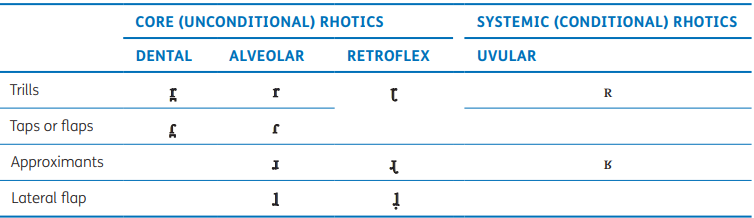
\includegraphics[scale=0.7]{rhotics.png}
    \caption{Rhotics list \citep[p.~4]{labrune2021word}}
    \label{fig:rhotics}
\end{figure}

``Avoidance'' is used instead of ``prohibition'' because, according to the author, the acceptance of rhotics in a language cannot always be answered with yes or no but is a matter of degree. An example given in the paper is that in a corpus of Maninka with over 28.000 tokens, rhotics appear 1564 times in total, but only 16 times in the initial position. The result of the paper is that 78 languages exhibit emic-WIRA and 30 languages exhibit etic-WIRA (nine of those also exhibit emic-WIRA). Since I will not investigate corpus in this thesis due to time restriction (and frequency data may not be mentioned in the descriptive grammar), the ``avoidance'' part is irrelevant to me.

\subsection{Language Sampling and WALS Sample List}

According to \citet{velupillai2012introduction}, there are three types of sampling used in typological studies: probability sampling, variety sampling, and convenience sampling. Probability sampling aims to be statistically representative, and thus tries to achieve genealogical and areal balance in the sample. Variety sampling aims to include as many variations as possible and thus may pay less attention to the genealogical or areal balance. Convenience sampling is, as its name, the sample that the researcher is able to access, though one can still try to be as diverse and representative as possible within it.

\par 
The World Atlas of Language Structures (WALS), while allowing the author of each chapter to choose the language sample they wish, provides a 100-language sample and a 200-language sample (built up on the 100-language sample) recommended to be included in every chapter \citep{wals-s1}. The 100 and 200 languages lists are constructed to maximize the diversity and to be representative of languages of the world, while also concerned with the availability of descriptive data on the languages. The languages of the 100-language sample are more well-known and have more detailed descriptions with better availability \citep{wals-s1}. Thus, the 100-language sample will be the starting point for constructing the 20-language sample in this thesis using semi-convenience sampling (more will be explained in the methodology).  

\subsection{Property-Driven Phonological Typology}

\citet{hyman2009not} claimed that there are two ways of doing typology: one focuses on classifying languages into ``types'', e.g. tone language and pitch-accent language, and the other focuses on specific properties of the language. The paper is also a criticism of language classification and advocates for focusing on properties instead (i.e. property-driven typology). In this thesis, I will not attempt language classification, that is, I will not put languages into a type like ``/\tipa{N}/ symmetric language'' or ``more symmetric language'' (based on the number of consonants that are symmetric in the language). I will only focus on the properties of each consonant in each language, the interest here are the segments themselves and not the languages that contain them. 

\par
Arguably, with this focus on the segment, it could be better to sample the segments and not the languages, i.e. investigate the distribution of 20 segments in all languages instead of all segments in 20 languages. However, the dimensions for segment sampling would be too large. For example, the ideal database for choosing 20 segments to investigate would be PHOIBLE \citep{phoible}, but for each segment, their presence would be counted in 3020 inventories of 2186 distinct languages. Within the scope of this thesis, that number would be impossible to work with, so I need to choose a more viable approach of sampling based on language.  

\chapter{Methodology}
\section{Language Sampling}

The sampling method I use is semi-convenience. It is ``semi-'', and not purely convenience, because the languages are chosen randomly from the 100-language sample of WALS. 
I draw a random 20-language list from the 100-language sample, then skim through the reference grammar of the language given in WALS to see if it contains the information I want. 
If the reference grammar is not accessible or it does not provide information on the consonantal distribution for the language, I attempt to find the data in other papers about the language. 
When that also fails, the language is replaced by another language (also chosen randomly from the 100-language sample) from a language family not already presented in the list.

\section{Data Treatment}

\subsection{Phonetics or Phonology?}

In works that consider the representation of phonology and phonetics in great depth like \citet{Boersma1998, Boersma2007}, phonology and phonetics is considered to have at least four levels: Underlying and Surface forms of phonology, and Articulatory and Auditory forms of phonetics.
Phonetic data, in the sense of acoustic signals and articulatory gestures, are probably the most `raw' data that can be used, while phonemes are already subjected to the analysis and perspective of the authors who wrote these grammars. 
Phonemic analysis can produce very different ways of categorizing sounds of a language, which may be justified for the language in question but may not fit for cross-linguistics comparison. 

\begin{figure}[h]
    \centering
    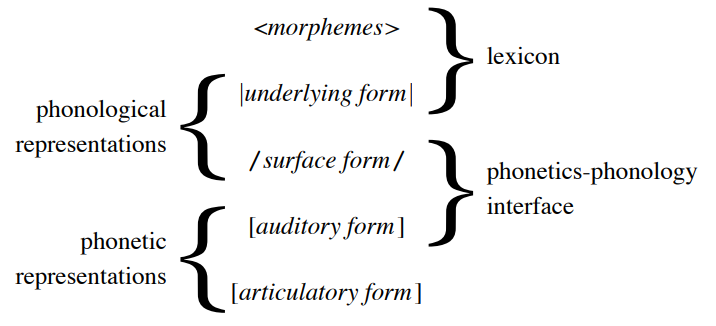
\includegraphics[width=0.75\linewidth]{figures/representation.png}
    \caption{Multi-level representation of phonetics and phonology \citep{Boersma2009}}
    \label{fig:representation}
\end{figure}

Ideally, I should have gathered data at the phonetic levels to have the primary data, but this task is impossible due to two problems.
The first problem is theoretical in that most reference grammars operate on the two levels model of phonetics-phonology: there are the Underlying Form (UF) of phonology, and Surface Form (SF) of phonetics. 
While their Underlying Form may correspond to Underlying Form in Figure \ref{fig:representation}, the degree of phonetic details in their Surface Form is unclear.
The second problem is more practical: most reference grammars do not focus on phonetic details, and so no phonetic data is available to gather from them. 
There are occasionally phonetic remarks, but those are scattered and not made in a systematic manner.

\par
Therefore, I decided to take a practical middle ground and record the data available at the allophonic level. 
For example, if English happens to be on my list then the `clear L' [l] and the `dark L' [ɫ] will be coded as two distinct sounds, with [l] only allowed in the onset, and [ɫ] only in the coda. 

\subsection{Bracket Notation}

The data collected and used in this paper resides, to some extent,between the boundary of phonetic and phonemic, so I have to make certain notation decisions.
In this paper, whenever I refer to the segments that I processed during data collection, I will use the square bracket `[]', since my aim is to record it at phonetic level.
The original reports from reference grammar may vary in terms of phonetic precision, but for the purpose of this paper I will consider them to be equal.
However, when referring to the segments that are used in the argument of other authors, I will respect their use of bracket.

\subsection{Cluster and segmentation}

Consonant clusters will not be considered in this thesis and individual segments in a cluster will be counted separately. However, I will respect the segmentation analysis of the author. Thus, if an author insists that, for instance, [ts] is one segment in this language, it will be coded as a sound distinct from both [t] and [s].

\subsection{Exclusion of certain allophonic variation}

Since the purpose of this thesis is to investigate the distributional asymmetry of consonants relative to the syllable, allophonic variations conditioned by other factors (e.g. as-/dis- similation) will be ignored. 
For example, if in a language, there are [tʃ] and [k] that are in complementary distribution where [tʃ] only appears before front vowels and [k] elsewhere, both of them will be recorded as one segment [k]. 

\par
This decision is not a statement about the real phonological representation of those segments, but merely a way to avoid confounding factors.
An alternative choice is to record both of them separately, but this could disturb the data on positional distribution.
For example, [tʃ] may ends up having higher count and especially in the initial position, because it is quite common to see /t/ and /k/ become [tʃ] in the surface form when followed by /i/ or /j/.
However, in this case the counting of [tʃ] in the initial position is caused partially by the proximity with a sound that has palatal constriction and not purely its position within a syllable.
Arguably, it could also be attributed to the position of the segment (assimilation in the initial position and not in final position), but then we may have to deal with anticipatory versus perseverative assimilation, which is far beyond the scope of this paper. 

\subsection{Data Encoding}

Three positions in the syllable will be distinguishedː initial, medial, and final. Initial and final means onset and coda, and medial means the intervocalic environment. 
If a segment is allowed in a position, it will be coded as 1, otherwise 0. However, if a language prohibits all final consonants, the segments will be coded as ``N/A'' for this position instead.

\par 
In my experience, sometimes the author writes nothing about intervocalic phonotactics. So, following the Maximal Onset Principle (MOP), if the author does not provide any information for the medial position, segments in this position will be assumed to share the same distribution with the initial position. This assumption does not mean that I believe MOP to be true, but it is a practical decision to fill in the gap in the data.

\begin{table}[h!]
    \centering
    \begin{tabular}{| l | l | l | l | l |}
    \hline
     Language & Segment & Initial & Medial & Final \\ \hline
	A & t & 1 & 1 & 1 \\ \hline
	A & d & 1 & 1 & 0 \\ \hline
	... &  &  &  &  \\ \hline
	Z & h & 1 & 0 & N/A \\ \hline
    \end{tabular}
    \caption{Example table}
    \label{tab:example}
\end{table}

\subsection{Data Analysis}

For each segment in each position the number of ``1'' will be divided by the sum of the number of ``1'' and ``0'', yielding a restriction percentage where 1.00 means not restricted while 0.00 means completely not allowed. 




\chapter{Result}
\section{Data}

\begin{table}[h]
\caption{The List of Languages}
\label{tab:language_list}
\resizebox{\textwidth}{!}{\begin{tabular}{|l|l|l|l|l|}
\hline
\textbf{code} & \textbf{Name}                                                          & \textbf{Genus}                                                                   & \textbf{Family}               & \textbf{Reference} \\ \hline
fij  & Fijian                                                        & Oceanic                                                                 & Austronesian         &    \citet{dixon1988grammar}       \\ \hline
tha  & Thai                                                          & Kam-Tai                                                                 & Tai-Kadai            &  \citet{tingsabadhThai1993}         \\ \hline
hau  & Hausa                                                         & West Chadic                                                             & Afro-Asiatic         &     \citet{newmanHausaLanguageEncyclopedic2000}      \\ \hline
lav  & Lavukaleve                                                    & Lavukaleve                                                              & Solomons East Papuan &        \citet{terrill2011grammar}   \\ \hline
qim  & \begin{tabular}[c]{@{}l@{}}Quechua \\ (Imbabura)\end{tabular} & Quechuan                                                                & Quechuan             &     \citet{coleImbaburaQuechua1985}      \\ \hline
may  & Maybrat                                                       & Maybrat                                                                 & Maybrat              &     \citet{dolGrammarMaybratLanguage2007}      \\ \hline
imo  & Imonda                                                        & Border                                                                  & Border               &      \citet{seilerImondaPapuanLanguage1985}     \\ \hline
kio  & Kiowa                                                         & Kiowa-Tanoan                                                            & Kiowa-Tanoan         &      \citet{watkinsGrammarKiowa1984}     \\ \hline
mnd  & Mandarin                                                      & Chinese                                                                 & Sino-Tibetan         &     \citet{liMandarinChineseFunctional2009}      \\ \hline
spa  & Spanish                                                       & Romance                                                                 & Indo-European        &      \citet{geeslinCambridgeHandbookSpanish2018}     \\ \hline
war  & Wari'                                                         & Chapacura-Wanham                                                        & Chapacura-Wanham     &      \citet{everettWari2002}     \\ \hline
kor  & Korean                                                        & Korean                                                                  & Korean               &     \citet{shinSoundsKorean2012}      \\ \hline
vie  & Vietnamese                                                    & Viet-Muong                                                              & Austro-Asiatic       &     \citet{kirbyVietnameseHanoiVietnamese2011}      \\ \hline
chk  & Chukchi                                                       & \begin{tabular}[c]{@{}l@{}}Northern \\ Chukotko-Kamchatkan\end{tabular} & Chukotko-Kamchatkan  &      \citet{dunnGrammarChukchi1999}     \\ \hline
wra  & Warao                                                         & Warao                                                                   & Warao                &      \citet{romero-figeroaReferenceGrammarWarao2003}     \\ \hline
knd  & Kannada                                                       & Dravidian                                                               & Dravidian            &      \citet{sridharKannada1990}     \\ \hline
sup  & Supyire                                                       & Senufo                                                                  & Niger-Congo          &     \citet{carlsonGrammarSupyire1994}      \\ \hline
tiw  & Tiwi                                                          & Tiwian                                                                  & Tiwian               &     \citet{osborneTiwiLanguageGrammar1974}      \\ \hline
lan  & Lango                                                         & Western Nilotic                                                         & Eastern Sudanic      &     \citet{noonanGrammarLango1992}      \\ \hline
kew  & Kewa                                                          & Enga\_Kewa-Huli                                                         & Trans-New Guinea     &     \citet{franklinGrammarKewaNew1971} \\ \hline
\end{tabular}}
\end{table}

The 20 languages used in this survey are presented in Table \ref{tab:language_list} along with their genealogical data and the reference used. 
A total of 411 tokens of 95 different segments was recorded, the 20 most common segments and their restriction percentages are presented in Table \ref{tab:segment_list}. The full list of all segments is provided in Appendix B. 

\begin{table}[]
\centering
\caption{List of most common segments}
\label{tab:segment_list}
\begin{tabular}{|l|l|l|l|l|}
\hline
Segment & Count & Initial & Medial & Final \\ \hline
m        & 20    & 1.00    & 1.00   & 0.94  \\ \hline
n        & 20    & 1.00    & 1.00   & 0.94  \\ \hline
t        & 20    & 1.00    & 0.90   & 0.56  \\ \hline
k        & 19    & 1.00    & 0.95   & 0.47  \\ \hline
p        & 18    & 0.94    & 0.89   & 0.43  \\ \hline
s        & 18    & 0.94    & 1.00   & 0.57  \\ \hline
l        & 16    & 0.94    & 0.94   & 0.62  \\ \hline
j        & 15    & 0.93    & 0.93   & 0.55  \\ \hline
d        & 13    & 0.92    & 0.85   & 0.20  \\ \hline
w        & 13    & 1.00    & 1.00   & 0.56  \\ \hline
b        & 12    & 0.92    & 0.92   & 0.30  \\ \hline
ŋ        & 12    & 0.67    & 0.67   & 1.00  \\ \hline
g        & 11    & 0.82    & 0.91   & 0.22  \\ \hline
f        & 10    & 1.00    & 0.90   & 0.63  \\ \hline
h        & 10    & 1.00    & 0.90   & 0.11  \\ \hline
r        & 10    & 0.90    & 1.00   & 0.57  \\ \hline
ɾ        & 8     & 0.63    & 1.00   & 0.71  \\ \hline
tʰ       & 8     & 0.88    & 0.88   & 0.25  \\ \hline
tʃ       & 7     & 1.00    & 1.00   & 0.00  \\ \hline
ʔ        & 7     & 0.86    & 1.00   & 0.40  \\ \hline
\end{tabular}
\end{table}

\section{Overview}
The list of 20 most frequent segments in this study is similar to the top 20 segments list reported in \citet[45]{Gordon_2016}, which comes from a survey of 317 languages. The only two different segments are [ʃ] and [ɲ] in his list compared to [r] and [tʰ] in my list. There are even some resemblance in terms of the frequency of each segmentsː [n t m k] are the four most common segments in both lists. Therefore, despite the small scale of this study the list of top 20 segments can still be considered representative of world languages to some degree. 

\par
For most segments in this survey, we can see that the distributional discrepancies between different positions are apparent. 
The most symmetric segments are [n] and [m], which have equal occurrences in initial and medial positions (20 languages), with slightly fewer instances in the final position (19 languages each). 
The distribution of velar nasal [ŋ] is consistent with the finding of \citet{wals-9}, namely that all languages that have [ŋ] allow it in the final position while only two-thirds of them allow it in the initial and medial position. 
Two most common ``rhotics'' in the data, [r] and [ɾ] also exhibit the Word-Initial Rhotic Avoidance to some degree, although it is more apparent for [ɾ] (63\% compared to 90\% of [r]).

\par
The non-continuant segments (i.e. with the oral tract completely blocked) in this study can be divided into three main groups: nasal, voiced stop and voiceless stop. 
It may be useful to discuss these segments together because all three major places of articulation (labial, coronal, and dorsal) of them appear in the top 20 most common segments of the study. 
In general, the nasal segments seem to be more symmetric than the voiceless, which in turn are more symmetric than the voiced.
The discrepancies lie mainly on the final position, since acceptance of them (except [ŋ]) is nearly 100\% in initial and medial position.
The voiced stop is the most restricted group in this position, only allowed in under one third of the languages in which they occur. 
They are followed by the voiceless stops, which is allowed in the final position for around a half of the languages that they appear in. 
The least restricted are the nasals, which are near universal also in the final position (100\% for [ŋ], and 94\% for each of [m] and [n]).


\par
Turning to the fricatives, we find three fricative segments in Table \ref{tab:segment_list}: [s], [f] and [h]. 
There is a large difference in the frequency of [s], which occurs in 18 languages compared to the other two fricatives, which occur in only 10 languages each. 
The behaviour of [s] and [f] are fairly similar to the voiceless stops. 
They are also near universal in the initial and medial position and  around 50\% in the final position
However, [s] appears slightly more favoured in the medial position than initial position. 
The glottal fricative [h], on the other hand, is much more restricted in the final position (only 11\%) while still having nearly universal acceptance in the other two positions.

\par
The non-nasal sonorants in Table \ref{tab:segment_list} are comprised of [l j w r ɾ]. 
Most of them behave similar to the voiceless stops, with near universal presence in the initial and medial, and around 50\% acceptance in final position. 
The exception is the rhotic tap [ɾ] which is much more restricted in the initial position while still universally accepted in the medial position. 
In fact initial is the most restricted position of [ɾ], even more than the final position. 
The final position of [ɾ], on the other hand, has the highest acceptance out of all non-nasal segments (71\%).

\par
The remaining miscellaneous segments are the aspirated stop [tʰ], the glottal stop [ʔ], and the affricate [tʃ]. 
The affricate is perhaps the most special segment out of the three. 
It is the only segment in Table \ref{tab:segment_list} that is totally inhibited from occurring in the final position. 
The glottal stop behaves similar to other (plain) voiceless stops while the voiceless aspirated [tʰ] behaves more like voiced stops.
Although also being voiceless, [tʰ] has lower acceptance than all other voiceless stops in all position, including the final.

\section{Discussion}

The non-continuants [m n ŋ p t k b d g] are very frequent in languages of the world, and as seen in Table \ref{tab:segment_list}, all of these segments also appear amongst the most common list.
So, I believe that we can start or discussion with these segments and their distribution.
I first discuss about the discrepancies between the onset-coda acceptance of nasals and obstruents and speculate some possible explanation.
Then, I will look at the distribution of the voiceless and voiced stop.

\par
The asymmetry between the set of segments that can occur in the onset and coda are well-known to linguists.
In the tradition of Optimality Theory (OT), there are two major markedness constraints regards syllable structure: \textsc{onset} and \textsc{nocoda}.
The first of them, \textsc{onset}, requires a syllable to have a consonantal onset, which is violated by vowel-initial syllable.
The \textsc{nocoda} constraint states that a syllable should not end with a consonant.
Thus, the syllables that have coda will violate the constraint and become less optimal than syllables without it.
According to OT, only the optimal form, meaning form that violates the least constraints, will be chosen to produce by the speaker.
Only when the faithfulness constraint is ranked above the markedness constraint that a syllable with coda in the underlying form can have its coda produced.
Therefore, it can be said that the 'default' option for syllable structure in languages is without a coda.
\citet{Gordon_2016} also reported a similar observation, that if a language permits syllables with coda, it will also permit syllables without coda.

\par
But it is clear from the data that not all coda are treated equally. 
If a language allows its syllable to have coda, the three nasals are almost universally a candidate for that position, while other segments are generally much less favoured.
Not all segments violate the \textsc{nocoda} constraint to the same degree, and there is some attribute of the nasals that make them violate the constraint to a lesser extend.
In \citet{Clements1990}, it is proposed that the syllable structure follows a Sonority Sequencing Principle, which states that the syllable typically only allows one sonority peak, usually a vowel, with sequences of consonants on their sides.
This principle also requires that the segments in the sequences have to be ordered, in term of sonority, in decreasing order toward the edges.  
The author observed that the initial and final of a syllable follow different generalization: while segments in the onset prefers to maximize their sonority difference from the nucleus, segments in the coda prefer minimizing their sonority difference. 
This means that if a language permits any coda at all, then the more sonorant codas (like nasals) are more preferred than their less sonorant counterparts (like stops).

\par
The difference in the restriction of voiced and voiceless stops can be expected by the well-known Final Obstruent Devoicing process. 
Final Obstruent Devoicing means that voiced stops can be neutralized to their voiceless counterpart when they are at the end of the word. 
Another related phenomena is Intervocalic Voicing where voiceless stop becomes voiced when it is between vowels. 
However, the predicted effect of this phenomena, namely that voiceless stops are more restricted than voiced stops in medial position, is not observed in the top 20 segments.
The likelihood of voiced and voiceless segments in medial position is found to be fairly equal.
This is quite surprising because some accounts consider them to be similar phonological processes, namely weakening processes \citep{Gordon_2016, harris2009final}.
Both can be seen as reducing the articulation effort: both abducting the vocal folds between two vowels to maintain voicing at the end of the word takes more effort \citep{Gordon_2016}. 
With these similarities between the two processes, it seems surprising why the effect of one is observed and the other is not.
Thus, the account of a weakening process is not enough to explain the distribution of voiced and voiceless segments in this data.

\par
It is possible that the efforts in the two cases are not the same and one has more priority than the other.
Indeed, voicing in vowels and consonants, although usually represented in phonology by the same feature, are different in terms of aerodynamic.
The voicing of vowels and sonorants is due to an absence of built-up air pressure in the oral tract while the voicing of obstruent requires such air pressure \citep{harris2009final}.
Thus, even when intervocalic voicing avoiding changing the adduction of the vocal folds (which is required for articulating vowels), it still has to increase the air pressure to make obstruent voicing possible.
So, intervocalic voicing can be seen as choosing between two efforts, changing the states of the vocal folds or increasing air pressure, while final devoicing only minimize efforts. 
That might be the reason why the preference for voicelessness of the stop in the final position is better reflected in the data.

\section{Interesting Findings}  

\subsection{The Glottal Stop}
The most phonetically favourable position for glottal stop is probably word-initial. 
Even languages like English, where glottal stop does not have phonemic status, still seem to favour word-initial glottal stop at the phonetic level \citep{garellekGlottalStop}. 
In fact, \citet{garellekGlottalStop} went as far as to suggest that perhaps all languages that does not contrast /\#V/ and /\#ʔV/ could insert [ʔ] at the beginning of the word, though they may do so with different degrees of frequency. Consider this in the context of the basics OT constraint \textsc{Onset}, the surface forms with [ʔ] in the onset would outrank the vowel-initial forms. 
Therefore, if a glottal stop exists in a language, it should be allowed in the initial position.

\par
However, the data gathered in Table \ref{tab:segment_list} shows that only seven of of the eight languages with glottal stop allow it in the initial position. 
The only language that does not allow initial glottal stop is Supyire, a language of the Niger-Congo family. 
This language's syllable structure is CV or CVV, with the exception of a few grammatical words that allow word-initial vowel \citep[7]{carlsonGrammarSupyire1994}. 
Given such syllable structure, one may expect that if the glottal stop is recognized in the language, its most favourable position would be word-initial.
However, the glottal stop is reported to be only a marginal phoneme in Supyire and can only appear in intervocalic environment. 
\citet{carlsonGrammarSupyire1994} speculated, based on evidence from loan words, that /ʔ/ (the author uses the symbol /h/) might be a reduction of an earlier /g/.
But because in the current phonological system of the language there is also a [g] that can appear in intervocalic position, I consider [ʔ] to be considered a separate phoneme instead of an allophone of [g].

\subsection{Final Avoidance of Two Nasals}

Although the nasals are supposed to be well-accepted in the final position, and the velar nasal is universally accepted, Table \ref{tab:segment_list} still shows two cases where /n/ or /m/ is not allowed in the coda. 
The first of them, the absence of /m/ in the coda, is observed in Mandarin Chinese.
The second one is the absence of final /n/, which is observed in Hausa, an Afro-Asiatic language.
The reason for the absence is different in each case: for Mandarin it is because of a historical merging process, while for Hausa it is allophony.

\par
The rhyme table for Mandarin Chinese presented in \citet{liMandarinChineseFunctional2009} contains only syllables that end with either a vowel or one of the two nasals [n] and [ŋ].
The labial nasal [m], despite being a legit segment in the onset, does not appear in the coda.
More surprisingly, /m/ is a legit segment in the coda in Middle Chinese, and still remain so in a few other Sinitic languages like Cantonese \citep{zee1985sound}. 
The explanation given by \citet{zee1985sound} is that the labial nasal /m/ has merged into /n/ in Mandarin Chinese.
Middle Chinese allowed all three nasals /m/, /n/ and /ŋ/ to appear in the end of the word, but there is a merging process that affects all Sinitic languages.
In this process, the labial nasal /m/ seems to be the prime target for being merged, and in Mandarin it is merged with /n/ \citep{zee1985sound}.

\par
For the case of Hausa, it is more due to methodological decision made in the process of data gathering. Specifically, \citet{newmanHausaLanguageEncyclopedic2000} presented Hausa as having only two phonemic nasals: /n/ and /m/. 
But he also noted that /n/ in the final position is always realized as [ŋ] and never as [n]. 
Therefore, in my data gathering Hausa is considered having both [n] and [ŋ], with [n] allowed in initial and medial and [ŋ] allowed in only final position.
The labial /m/ is also usually realized as [ŋ], but there are some cases where it is still realized as [m].
Thus, [m] is still coded as being allowed in all three position in my data.

\par
Thus, the absence of word-final /m/ in Mandarin and /n/ in Hausa is not an evidence against the universal acceptance of nasals in word-final position.
They are some particular cases of historical changes or allophony within the space of the nasal inventory.
But another interesting question that they pose is "Why the velar nasal?".
Although in Mandarin /n/ still remain distinguished from /ŋ/, some other Sinitic languages also show a process of /n/ merging to /ŋ/ \citet{zee1985sound}.
Combined that with the distribution of /ŋ/ in word-final position, as observed in \citet{wals-9}, it seems like the velar nasal holds a strong preference in this position.
One possible speculation is that the velar nasal is the most vowel-like nasal.
And if it is true that languages prefer to end words with a vowel, then the velar nasal could be the most highly ranked alternative.


\chapter{Conclusion}
Despite the small language list used in this study, and thus the lack of significant statistical analysis, a few patterns can be observed from the data of the 20 most common segments.
We can first conclude that asymmetry is indeed the norm for most segments, with the exception of two nasals /n/ and /m/.
The nasals, if they exist in a language, are always allowed in the final position.
Two of them, /m/ and /n/, are also always allowed in the initial and medial position.
There are two cases where /m/ and /n/ are absent from the final position but they are due to a process of merging or allophony with another common nasals.
The velar nasal /ŋ/, on the other hand, is only universally allowed in the final position and is more restricted in other position.
While this observation conforms to the report from \cite{wals-9}, neither the fact that the distribution of /ŋ/ is asymmetric nor its degree of asymmetry is special.
However, what makes the distribution of /ŋ/ special is that it is the only segment that is skewed toward the final position.

\par
One particular question that remains is why the nasals are that well-accepted in the final position, and a possible reason could be due to its high sonority.
But that answer is still unsatisfying since other sonorants like liquids and glides are just as popular in the final position as the voiceless stops, which is on the other end of the sonority scale.
Perhaps the nasals are more similar to vowels than other sonorants in some attributes that are not considered in this thesis.

\par
Turning to the voiced and voiceless stops, the strong restriction on the voiced stops in the final position is well-expected by the Final Obstruent Avoidance process.
However, the effect of the related phenomena of intervocalic voicing is not observed in the data.
A speculated explanation is that maintaining voicing in word-final position takes more effort than keeping the stops voiceless between two vowels.
Therefore, the need to avoid voicing in word-final stops is more profound and reflected better in the data.

\par
Due to numerous limitation, many explanations of the data in this study have to remain at the speculation stage.
Nevertheless, it can serve as a preliminary research to look for direction for further studies.
For example, another research could try to compare the similarity between vowels and nasals versus vowels and other sonorants as a way to explain the high acceptance of nasals in word-final position.


\appendix
\chapter{Full Distribution Table}
\renewcommand{\arraystretch}{1.2}
\begin{longtable}{ | l | l | l | l | l | }
\hline
	Language & Segment & Initial & Medial & Final \\ \hline
	fij & m & 1 & 1 & N/A \\ \hline
	fij & p & 1 & 1 & N/A \\ \hline
	fij & mb & 1 & 1 & N/A \\ \hline
	fij & β & 1 & 1 & N/A \\ \hline
	fij & f & 1 & 1 & N/A \\ \hline
	fij & n & 1 & 1 & N/A \\ \hline
	fij & t & 1 & 1 & N/A \\ \hline
	fij & nd & 1 & 1 & N/A \\ \hline
	fij & ð & 1 & 1 & N/A \\ \hline
	fij & r & 1 & 1 & N/A \\ \hline
	fij & nr & 1 & 1 & N/A \\ \hline
	fij & s & 1 & 1 & N/A \\ \hline
	fij & tʃ & 1 & 1 & N/A \\ \hline
	fij & l & 1 & 1 & N/A \\ \hline
	fij & j & 1 & 1 & N/A \\ \hline
	fij & ŋ & 1 & 1 & N/A \\ \hline
	fij & k & 1 & 1 & N/A \\ \hline
	fij & ŋg & 1 & 1 & N/A \\ \hline
	fij & w & 1 & 1 & N/A \\ \hline
	fij & ʔ & 1 & 1 & N/A \\ \hline
	lav & pʰ & 1 & 1 & 0 \\ \hline
	lav & tʰ & 1 & 1 & 1 \\ \hline
	lav & t & 1 & 0 & 0 \\ \hline
	lav & kʰ & 1 & 1 & 1 \\ \hline
	lav & b & 1 & 1 & 0 \\ \hline
	lav & mb & 0 & 1 & 0 \\ \hline
	lav & d & 1 & 1 & 0 \\ \hline
	lav & nd & 0 & 1 & 0 \\ \hline
	lav & m & 1 & 1 & 1 \\ \hline
	lav & n & 1 & 1 & 1 \\ \hline
	lav & ŋ & 1 & 1 & 1 \\ \hline
	lav & r & 1 & 1 & 1 \\ \hline
	lav & l & 1 & 1 & 1 \\ \hline
	lav & f & 1 & 1 & 1 \\ \hline
	lav & s & 1 & 1 & 1 \\ \hline
	lav & h & 1 & 1 & 0 \\ \hline
	lav & β & 1 & 1 & 1 \\ \hline
	lav & ɰ & 1 & 1 & 1 \\ \hline
	qim & p & 1 & 1 & 0 \\ \hline
	qim & t & 1 & 1 & 0 \\ \hline
	qim & k & 1 & 1 & 0 \\ \hline
	qim & ts & 1 & 1 & 0 \\ \hline
	qim & tʃ & 1 & 1 & 0 \\ \hline
	qim & b & 1 & 1 & 0 \\ \hline
	qim & d & 1 & 1 & 0 \\ \hline
	qim & g & 1 & 1 & 0 \\ \hline
	qim & ɸ & 1 & 1 & 0 \\ \hline
	qim & s & 1 & 1 & 1 \\ \hline
	qim & ʃ & 1 & 1 & 1 \\ \hline
	qim & x & 1 & 1 & 1 \\ \hline
	qim & β & 1 & 1 & 0 \\ \hline
	qim & z & 1 & 1 & 0 \\ \hline
	qim & ʒ & 1 & 1 & 0 \\ \hline
	qim & m & 1 & 1 & 1 \\ \hline
	qim & n & 1 & 1 & 1 \\ \hline
	qim & ɲ & 1 & 1 & 0 \\ \hline
	qim & ŋ & 0 & 0 & 1 \\ \hline
	qim & l & 1 & 1 & 1 \\ \hline
	qim & ʐ & 1 & 0 & 0 \\ \hline
	qim & ɾ & 0 & 1 & 1 \\ \hline
	qim & w & 1 & 1 & 1 \\ \hline
	qim & j & 1 & 1 & 1 \\ \hline
	may & p & 1 & 1 & 0 \\ \hline
	may & t & 1 & 1 & 1 \\ \hline
	may & tʰ & 0 & 0 & 1 \\ \hline
	may & t̚ & 0 & 0 & 1 \\ \hline
	may & k & 1 & 1 & 1 \\ \hline
	may & g & 0 & 1 & 0 \\ \hline
	may & k̚ & 0 & 0 & 1 \\ \hline
	may & m & 1 & 1 & 1 \\ \hline
	may & n & 1 & 1 & 1 \\ \hline
	may & f & 1 & 1 & 1 \\ \hline
	may & s & 1 & 1 & 1 \\ \hline
	may & x & 1 & 1 & 1 \\ \hline
	may & r & 1 & 1 & 1 \\ \hline
	may & ɾ & 0 & 1 & 1 \\ \hline
	may & w & 1 & 1 & 0 \\ \hline
	may & j & 1 & 1 & 0 \\ \hline
	imo & f & 1 & 0 & 1 \\ \hline
	imo & v & 0 & 1 & 0 \\ \hline
	imo & p & 1 & 1 & 0 \\ \hline
	imo & b & 1 & 0 & 0 \\ \hline
	imo & mb & 0 & 1 & 1 \\ \hline
	imo & m & 1 & 1 & 1 \\ \hline
	imo & n & 1 & 1 & 1 \\ \hline
	imo & s & 1 & 1 & 1 \\ \hline
	imo & l & 1 & 1 & 1 \\ \hline
	imo & t & 1 & 1 & 1 \\ \hline
	imo & d & 1 & 0 & 0 \\ \hline
	imo & nd & 0 & 1 & 1 \\ \hline
	imo & k & 1 & 1 & 1 \\ \hline
	imo & g & 1 & 0 & 0 \\ \hline
	imo & ŋg & 0 & 1 & 1 \\ \hline
	imo & h & 1 & 1 & 1 \\ \hline
	imo & ɦ & 0 & 1 & 0 \\ \hline
	kio & p & 1 & 1 & 1 \\ \hline
	kio & pʼ & 1 & 1 & 0 \\ \hline
	kio & pʰ & 1 & 1 & 0 \\ \hline
	kio & b & 1 & 1 & 0 \\ \hline
	kio & m & 1 & 1 & 1 \\ \hline
	kio & t & 1 & 1 & 1 \\ \hline
	kio & tʼ & 1 & 1 & 0 \\ \hline
	kio & tʰ & 1 & 1 & 0 \\ \hline
	kio & d & 1 & 1 & 0 \\ \hline
	kio & n & 1 & 1 & 1 \\ \hline
	kio & l & 1 & 1 & 0 \\ \hline
	kio & ᵈl & 0 & 0 & 1 \\ \hline
	kio & ts & 1 & 1 & 0 \\ \hline
	kio & tsʼ & 1 & 1 & 0 \\ \hline
	kio & s & 1 & 1 & 0 \\ \hline
	kio & z & 1 & 1 & 0 \\ \hline
	kio & j & 1 & 1 & 1 \\ \hline
	kio & k & 1 & 1 & 0 \\ \hline
	kio & kʼ & 1 & 1 & 0 \\ \hline
	kio & kʰ & 1 & 1 & 0 \\ \hline
	kio & g & 1 & 1 & 0 \\ \hline
	kio & h & 1 & 1 & 0 \\ \hline
	mnd & p & 1 & 1 & 0 \\ \hline
	mnd & pʰ & 1 & 1 & 0 \\ \hline
	mnd & t & 1 & 1 & 0 \\ \hline
	mnd & tʰ & 1 & 1 & 0 \\ \hline
	mnd & k & 1 & 1 & 0 \\ \hline
	mnd & kʰ & 1 & 1 & 0 \\ \hline
	mnd & ts & 1 & 1 & 0 \\ \hline
	mnd & tʂ & 1 & 1 & 0 \\ \hline
	mnd & tɕ & 1 & 1 & 0 \\ \hline
	mnd & tsʰ & 1 & 1 & 0 \\ \hline
	mnd & tʂʰ & 1 & 1 & 0 \\ \hline
	mnd & tɕʰ & 1 & 1 & 0 \\ \hline
	mnd & m & 1 & 1 & 0 \\ \hline
	mnd & n & 1 & 1 & 1 \\ \hline
	mnd & f & 1 & 1 & 0 \\ \hline
	mnd & s & 1 & 1 & 0 \\ \hline
	mnd & ʂ & 1 & 1 & 0 \\ \hline
	mnd & ɕ & 1 & 1 & 0 \\ \hline
	mnd & x & 1 & 1 & 0 \\ \hline
	mnd & l & 1 & 1 & 0 \\ \hline
	mnd & ɹ & 1 & 1 & 0 \\ \hline
	mnd & ŋ & 0 & 0 & 1 \\ \hline
	spa & p & 1 & 1 & 1 \\ \hline
	spa & b & 1 & 1 & 1 \\ \hline
	spa & m & 1 & 1 & 1 \\ \hline
	spa & f & 1 & 1 & 1 \\ \hline
	spa & θ & 1 & 1 & 1 \\ \hline
	spa & t & 1 & 1 & 1 \\ \hline
	spa & d & 1 & 1 & 1 \\ \hline
	spa & s & 1 & 1 & 1 \\ \hline
	spa & n & 1 & 1 & 1 \\ \hline
	spa & l & 1 & 1 & 1 \\ \hline
	spa & ɾ & 1 & 1 & 1 \\ \hline
	spa & r & 1 & 1 & 1 \\ \hline
	spa & tʃ & 1 & 1 & 0 \\ \hline
	spa & ɲ & 1 & 1 & 0 \\ \hline
	spa & ɟ & 1 & 1 & 1 \\ \hline
	spa & ʎ & 1 & 1 & 0 \\ \hline
	spa & k & 1 & 1 & 1 \\ \hline
	spa & g & 1 & 1 & 1 \\ \hline
	spa & x & 1 & 1 & 1 \\ \hline
	war & p & 1 & 1 & 0 \\ \hline
	war & p̚ & 0 & 0 & 1 \\ \hline
	war & t & 1 & 1 & 0 \\ \hline
	war & t̚ & 0 & 0 & 1 \\ \hline
	war & tʙ̊ & 1 & 1 & 0 \\ \hline
	war & k & 1 & 1 & 0 \\ \hline
	war & k̚ & 0 & 0 & 1 \\ \hline
	war & kʷ & 1 & 1 & 0 \\ \hline
	war & ʔ & 1 & 1 & 1 \\ \hline
	war & tʃ & 1 & 1 & 0 \\ \hline
	war & h & 1 & 1 & 0 \\ \hline
	war & m & 1 & 1 & 1 \\ \hline
	war & mb & 1 & 1 & 0 \\ \hline
	war & mʔ & 0 & 0 & 1 \\ \hline
	war & n & 1 & 1 & 1 \\ \hline
	war & nd & 1 & 1 & 0 \\ \hline
	war & nʔ & 0 & 0 & 1 \\ \hline
	war & ɾ & 1 & 1 & 0 \\ \hline
	war & w & 1 & 1 & 0 \\ \hline
	war & j & 1 & 1 & 0 \\ \hline
	kor & p & 1 & 0 & 0 \\ \hline
	kor & p͈ & 1 & 1 & 0 \\ \hline
	kor & pʰ & 1 & 1 & 0 \\ \hline
	kor & p̚ & 0 & 0 & 1 \\ \hline
	kor & b & 0 & 1 & 0 \\ \hline
	kor & t & 1 & 0 & 0 \\ \hline
	kor & t͈ & 1 & 1 & 0 \\ \hline
	kor & tʰ & 1 & 1 & 0 \\ \hline
	kor & t̚ & 0 & 0 & 1 \\ \hline
	kor & d & 0 & 1 & 0 \\ \hline
	kor & k & 1 & 0 & 0 \\ \hline
	kor & k͈ & 1 & 1 & 0 \\ \hline
	kor & kʰ & 1 & 1 & 0 \\ \hline
	kor & k̚ & 0 & 0 & 1 \\ \hline
	kor & g & 0 & 1 & 0 \\ \hline
	kor & s & 1 & 1 & 0 \\ \hline
	kor & s͈ & 1 & 1 & 0 \\ \hline
	kor & h & 1 & 0 & 0 \\ \hline
	kor & ɦ & 0 & 1 & 0 \\ \hline
	kor & tɕ & 1 & 0 & 0 \\ \hline
	kor & dʑ & 0 & 1 & 0 \\ \hline
	kor & tɕ͈ & 1 & 1 & 0 \\ \hline
	kor & tɕʰ & 1 & 1 & 0 \\ \hline
	kor & m & 1 & 1 & 1 \\ \hline
	kor & n & 1 & 1 & 1 \\ \hline
	kor & ŋ & 0 & 0 & 1 \\ \hline
	kor & l & 0 & 0 & 1 \\ \hline
	kor & ɾ & 1 & 1 & 0 \\ \hline
	vie & ɓ & 1 & 1 & 0 \\ \hline
	vie & p & 0 & 0 & 1 \\ \hline
	vie & m & 1 & 1 & 1 \\ \hline
	vie & w & 1 & 1 & 1 \\ \hline
	vie & f & 1 & 1 & 0 \\ \hline
	vie & v & 1 & 1 & 0 \\ \hline
	vie & t & 1 & 1 & 1 \\ \hline
	vie & tʰ & 1 & 1 & 0 \\ \hline
	vie & n & 1 & 1 & 1 \\ \hline
	vie & l & 1 & 1 & 0 \\ \hline
	vie & ɗ & 1 & 1 & 0 \\ \hline
	vie & s & 1 & 1 & 0 \\ \hline
	vie & z & 1 & 1 & 0 \\ \hline
	vie & tɕ & 1 & 1 & 0 \\ \hline
	vie & ɲ & 1 & 1 & 0 \\ \hline
	vie & j & 0 & 0 & 1 \\ \hline
	vie & k & 1 & 1 & 1 \\ \hline
	vie & ŋ & 1 & 1 & 1 \\ \hline
	vie & x & 1 & 1 & 0 \\ \hline
	vie & ɣ & 1 & 1 & 0 \\ \hline
	vie & ʔ & 1 & 1 & 0 \\ \hline
	vie & h & 1 & 1 & 0 \\ \hline
	chk & p & 1 & 1 & 1 \\ \hline
	chk & m & 1 & 1 & 1 \\ \hline
	chk & w & 1 & 1 & 1 \\ \hline
	chk & t & 1 & 1 & 1 \\ \hline
	chk & n & 1 & 1 & 1 \\ \hline
	chk & ɾ & 1 & 1 & 1 \\ \hline
	chk & s & 1 & 1 & 1 \\ \hline
	chk & ɬ & 1 & 1 & 1 \\ \hline
	chk & j & 1 & 1 & 1 \\ \hline
	chk & k & 1 & 1 & 1 \\ \hline
	chk & ŋ & 1 & 1 & 1 \\ \hline
	chk & ɣ & 1 & 1 & 1 \\ \hline
	chk & q & 1 & 1 & 1 \\ \hline
	wra & p & 1 & 1 & N/A \\ \hline
	wra & m & 1 & 1 & N/A \\ \hline
	wra & w & 1 & 1 & N/A \\ \hline
	wra & t & 1 & 1 & N/A \\ \hline
	wra & s & 1 & 1 & N/A \\ \hline
	wra & r & 0 & 1 & N/A \\ \hline
	wra & d & 1 & 0 & N/A \\ \hline
	wra & n & 1 & 1 & N/A \\ \hline
	wra & j & 1 & 1 & N/A \\ \hline
	wra & k & 1 & 1 & N/A \\ \hline
	wra & kʷ & 1 & 1 & N/A \\ \hline
	wra & h & 1 & 1 & N/A \\ \hline
	knd & p & 1 & 1 & 0 \\ \hline
	knd & pʰ & 1 & 1 & 0 \\ \hline
	knd & b & 1 & 1 & 0 \\ \hline
	knd & bʰ & 1 & 1 & 0 \\ \hline
	knd & t & 1 & 1 & 0 \\ \hline
	knd & tʰ & 1 & 1 & 0 \\ \hline
	knd & d & 1 & 1 & 0 \\ \hline
	knd & dʰ & 1 & 1 & 0 \\ \hline
	knd & ʈ & 1 & 1 & 0 \\ \hline
	knd & ʈʰ & 1 & 1 & 0 \\ \hline
	knd & ɖ & 1 & 1 & 0 \\ \hline
	knd & ɖʰ & 0 & 1 & 0 \\ \hline
	knd & k & 1 & 1 & 0 \\ \hline
	knd & kʰ & 1 & 1 & 0 \\ \hline
	knd & g & 1 & 1 & 0 \\ \hline
	knd & gʰ & 1 & 1 & 0 \\ \hline
	knd & tʃ & 1 & 1 & 0 \\ \hline
	knd & dʒ & 1 & 1 & 1 \\ \hline
	knd & f & 1 & 1 & 1 \\ \hline
	knd & s & 1 & 1 & 1 \\ \hline
	knd & z & 1 & 1 & 0 \\ \hline
	knd & ʃ & 1 & 1 & 0 \\ \hline
	knd & ʂ & 1 & 1 & 0 \\ \hline
	knd & m & 1 & 1 & 1 \\ \hline
	knd & n & 1 & 1 & 1 \\ \hline
	knd & ɳ & 0 & 1 & 0 \\ \hline
	knd & l & 1 & 1 & 0 \\ \hline
	knd & ɭ & 1 & 1 & 0 \\ \hline
	knd & r & 1 & 1 & 0 \\ \hline
	knd & j & 1 & 1 & 0 \\ \hline
	knd & v & 1 & 1 & 0 \\ \hline
	sup & p & 1 & 1 & N/A \\ \hline
	sup & b & 1 & 1 & N/A \\ \hline
	sup & f & 1 & 1 & N/A \\ \hline
	sup & v & 1 & 1 & N/A \\ \hline
	sup & m & 1 & 1 & N/A \\ \hline
	sup & t & 1 & 1 & N/A \\ \hline
	sup & d & 1 & 1 & N/A \\ \hline
	sup & ɾ & 0 & 1 & N/A \\ \hline
	sup & s & 1 & 1 & N/A \\ \hline
	sup & z & 1 & 1 & N/A \\ \hline
	sup & n & 1 & 1 & N/A \\ \hline
	sup & l & 1 & 1 & N/A \\ \hline
	sup & tʃ & 1 & 1 & N/A \\ \hline
	sup & dʒ & 1 & 1 & N/A \\ \hline
	sup & ʃ & 1 & 1 & N/A \\ \hline
	sup & ʒ & 1 & 1 & N/A \\ \hline
	sup & ɲ & 1 & 1 & N/A \\ \hline
	sup & j & 1 & 1 & N/A \\ \hline
	sup & k & 1 & 1 & N/A \\ \hline
	sup & g & 1 & 1 & N/A \\ \hline
	sup & ʀ & 0 & 1 & N/A \\ \hline
	sup & ŋ & 1 & 1 & N/A \\ \hline
	sup & w & 1 & 1 & N/A \\ \hline
	sup & ʔ & 0 & 1 & N/A \\ \hline
	tiw & p & 1 & 1 & 0 \\ \hline
	tiw & m & 1 & 1 & 1 \\ \hline
	tiw & t̪ & 1 & 1 & 0 \\ \hline
	tiw & n̪ & 1 & 1 & 1 \\ \hline
	tiw & j & 1 & 1 & 0 \\ \hline
	tiw & t & 1 & 1 & 0 \\ \hline
	tiw & n & 1 & 1 & 1 \\ \hline
	tiw & l & 1 & 1 & 1 \\ \hline
	tiw & r & 1 & 1 & 0 \\ \hline
	tiw & ɹ & 1 & 1 & 1 \\ \hline
	tiw & k & 1 & 1 & 0 \\ \hline
	tiw & ŋ & 1 & 1 & 1 \\ \hline
	tiw & ɣ & 1 & 1 & 0 \\ \hline
	tiw & w & 1 & 1 & 0 \\ \hline
	lan & p & 1 & 1 & 1 \\ \hline
	lan & t & 1 & 1 & 1 \\ \hline
	lan & tɕ & 1 & 1 & 1 \\ \hline
	lan & k & 1 & 1 & 1 \\ \hline
	lan & b & 1 & 1 & 1 \\ \hline
	lan & d & 1 & 1 & 1 \\ \hline
	lan & dʑ & 1 & 1 & 1 \\ \hline
	lan & g & 1 & 1 & 1 \\ \hline
	lan & m & 1 & 1 & 1 \\ \hline
	lan & n & 1 & 1 & 1 \\ \hline
	lan & ɲ & 1 & 1 & 1 \\ \hline
	lan & ŋ & 1 & 1 & 1 \\ \hline
	lan & ɸ & 0 & 1 & 0 \\ \hline
	lan & s & 0 & 1 & 0 \\ \hline
	lan & ɕ & 0 & 1 & 0 \\ \hline
	lan & x & 0 & 1 & 0 \\ \hline
	lan & ɾ̥ & 0 & 1 & 0 \\ \hline
	lan & ɾ & 1 & 1 & 1 \\ \hline
	lan & l & 1 & 1 & 1 \\ \hline
	lan & j & 1 & 1 & 0 \\ \hline
	lan & w & 1 & 1 & 0 \\ \hline
	lan & ʔ & 1 & 1 & 0 \\ \hline
	kew & p & 1 & 1 & N/A \\ \hline
	kew & t & 1 & 1 & N/A \\ \hline
	kew & k & 1 & 1 & N/A \\ \hline
	kew & b & 1 & 1 & N/A \\ \hline
	kew & d & 1 & 1 & N/A \\ \hline
	kew & g & 1 & 1 & N/A \\ \hline
	kew & m & 1 & 1 & N/A \\ \hline
	kew & n & 1 & 1 & N/A \\ \hline
	kew & l & 1 & 1 & N/A \\ \hline
	kew & r & 1 & 1 & N/A \\ \hline
	kew & s & 1 & 1 & N/A \\ \hline
	kew & w & 1 & 1 & N/A \\ \hline
	kew & j & 1 & 1 & N/A \\ \hline
	tha & p & 1 & 1 & 1 \\ \hline
	tha & b & 1 & 1 & 0 \\ \hline
	tha & pʰ & 1 & 1 & 0 \\ \hline
	tha & t & 1 & 1 & 1 \\ \hline
	tha & d & 1 & 1 & 0 \\ \hline
	tha & tʰ & 1 & 1 & 0 \\ \hline
	tha & k & 1 & 1 & 1 \\ \hline
	tha & kʰ & 1 & 1 & 0 \\ \hline
	tha & ʔ & 1 & 1 & 1 \\ \hline
	tha & m & 1 & 1 & 1 \\ \hline
	tha & n & 1 & 1 & 1 \\ \hline
	tha & ŋ & 1 & 1 & 1 \\ \hline
	tha & f & 1 & 1 & 0 \\ \hline
	tha & s & 1 & 1 & 0 \\ \hline
	tha & h & 1 & 1 & 0 \\ \hline
	tha & tɕ & 1 & 1 & 0 \\ \hline
	tha & tɕʰ & 1 & 1 & 0 \\ \hline
	tha & r & 1 & 1 & 0 \\ \hline
	tha & j & 1 & 1 & 1 \\ \hline
	tha & w & 1 & 1 & 1 \\ \hline
	tha & l & 1 & 1 & 0 \\ \hline
	tha & h & 1 & 1 & 0 \\ \hline
	hau & b & 1 & 1 & 1 \\ \hline
	hau & ɓ & 1 & 1 & 1 \\ \hline
	hau & m & 1 & 1 & 1 \\ \hline
	hau & ɸ & 1 & 1 & 1 \\ \hline
	hau & w & 1 & 1 & 1 \\ \hline
	hau & t & 1 & 1 & 1 \\ \hline
	hau & d & 1 & 1 & 0 \\ \hline
	hau & tsʼ & 1 & 1 & 0 \\ \hline
	hau & ɗ & 1 & 1 & 0 \\ \hline
	hau & n & 1 & 1 & 0 \\ \hline
	hau & ŋ & 0 & 0 & 1 \\ \hline
	hau & s & 1 & 1 & 1 \\ \hline
	hau & z & 1 & 1 & 1 \\ \hline
	hau & r & 1 & 1 & 1 \\ \hline
	hau & ɽ & 1 & 1 & 1 \\ \hline
	hau & l & 1 & 1 & 1 \\ \hline
	hau & tʃ & 1 & 1 & 0 \\ \hline
	hau & dʒ & 1 & 1 & 0 \\ \hline
	hau & ʔʲ & 1 & 1 & 0 \\ \hline
	hau & ʃ & 1 & 1 & 0 \\ \hline
	hau & j & 1 & 1 & 1 \\ \hline
	hau & k & 1 & 1 & 0 \\ \hline
	hau & g & 1 & 1 & 0 \\ \hline
	hau & kʼ & 1 & 1 & 0 \\ \hline
	hau & kʲ & 1 & 1 & 0 \\ \hline
	hau & gʲ & 1 & 1 & 0 \\ \hline
	hau & kʲʼ & 1 & 1 & 0 \\ \hline
	hau & kʷ & 1 & 1 & 0 \\ \hline
	hau & gʷ & 1 & 1 & 0 \\ \hline
	hau & kʷʼ & 1 & 1 & 0 \\ \hline
	hau & ʔ & 1 & 1 & 0 \\ \hline
	hau & h & 1 & 1 & 0 \\ \hline
\end{longtable}

\chapter{Full List of Segments}
\begin{longtable}{|l|l|l|l|l|}
\hline
Segment & Count & Initial & Medial & Final \\ \hline
n       & 20    & 1.00    & 1.00   & 0.88  \\ \hline
t       & 20    & 1.00    & 0.90   & 0.53  \\ \hline
m       & 20    & 1.00    & 1.00   & 0.88  \\ \hline
k       & 19    & 1.00    & 0.95   & 0.44  \\ \hline
s       & 18    & 0.94    & 1.00   & 0.53  \\ \hline
p       & 18    & 0.94    & 0.89   & 0.40  \\ \hline
l       & 16    & 0.94    & 0.94   & 0.57  \\ \hline
j       & 15    & 0.93    & 0.93   & 0.50  \\ \hline
w       & 13    & 1.00    & 1.00   & 0.50  \\ \hline
d       & 13    & 0.92    & 0.85   & 0.18  \\ \hline
b       & 12    & 0.92    & 0.92   & 0.27  \\ \hline
ŋ       & 12    & 0.67    & 0.67   & 1.00  \\ \hline
g       & 11    & 0.82    & 0.91   & 0.20  \\ \hline
h       & 10    & 1.00    & 0.90   & 0.11  \\ \hline
f       & 10    & 1.00    & 0.90   & 0.63  \\ \hline
r       & 10    & 0.90    & 1.00   & 0.50  \\ \hline
tʰ      & 8     & 0.88    & 0.88   & 0.25  \\ \hline
ɾ       & 8     & 0.63    & 1.00   & 0.71  \\ \hline
tʃ      & 7     & 1.00    & 1.00   & 0.00  \\ \hline
ʔ       & 7     & 0.86    & 1.00   & 0.40  \\ \hline
x       & 6     & 0.83    & 1.00   & 0.50  \\ \hline
pʰ      & 6     & 1.00    & 1.00   & 0.00  \\ \hline
z       & 6     & 1.00    & 1.00   & 0.20  \\ \hline
kʰ      & 6     & 1.00    & 1.00   & 0.17  \\ \hline
ɲ       & 5     & 1.00    & 1.00   & 0.25  \\ \hline
tɕ      & 5     & 1.00    & 0.80   & 0.20  \\ \hline
v       & 4     & 0.75    & 1.00   & 0.00  \\ \hline
mb      & 4     & 0.50    & 1.00   & 0.33  \\ \hline
ʃ       & 4     & 1.00    & 1.00   & 0.33  \\ \hline
dʒ      & 3     & 1.00    & 1.00   & 0.50  \\ \hline
kʷ      & 3     & 1.00    & 1.00   & 0.00  \\ \hline
ⁿd      & 3     & 0.33    & 1.00   & 0.50  \\ \hline
tɕʰ     & 3     & 1.00    & 1.00   & 0.00  \\ \hline
ɣ       & 3     & 1.00    & 1.00   & 0.33  \\ \hline
k̚      & 3     & 0.00    & 0.00   & 1.00  \\ \hline
t̚      & 3     & 0.00    & 0.00   & 1.00  \\ \hline
ts      & 3     & 1.00    & 1.00   & 0.00  \\ \hline
β       & 3     & 1.00    & 1.00   & 0.50  \\ \hline
ɸ       & 3     & 0.67    & 1.00   & 0.33  \\ \hline
ʂ       & 2     & 1.00    & 1.00   & 0.00  \\ \hline
ɗ       & 2     & 1.00    & 1.00   & 0.00  \\ \hline
ɓ       & 2     & 1.00    & 1.00   & 0.50  \\ \hline
ᵑg      & 2     & 0.50    & 1.00   & 1.00  \\ \hline
dʑ      & 2     & 0.50    & 1.00   & 0.50  \\ \hline
p̚      & 2     & 0.00    & 0.00   & 1.00  \\ \hline
ʒ       & 2     & 1.00    & 1.00   & 0.00  \\ \hline
ɕ       & 2     & 0.50    & 1.00   & 0.00  \\ \hline
tsʼ     & 2     & 1.00    & 1.00   & 0.00  \\ \hline
kʼ      & 2     & 1.00    & 1.00   & 0.00  \\ \hline
ɹ       & 2     & 1.00    & 1.00   & 0.50  \\ \hline
ɦ       & 2     & 0.00    & 1.00   & 0.00  \\ \hline
tsʰ     & 1     & 1.00    & 1.00   & 0.00  \\ \hline
tɕ͈     & 1     & 1.00    & 1.00   & 0.00  \\ \hline
ɳ       & 1     & 0.00    & 1.00   & 0.00  \\ \hline
p͈      & 1     & 1.00    & 1.00   & 0.00  \\ \hline
bʰ      & 1     & 1.00    & 1.00   & 0.00  \\ \hline
ɖʰ      & 1     & 0.00    & 1.00   & 0.00  \\ \hline
pʼ      & 1     & 1.00    & 1.00   & 0.00  \\ \hline
n̪      & 1     & 1.00    & 1.00   & 1.00  \\ \hline
tʙ̊     & 1     & 1.00    & 1.00   & 0.00  \\ \hline
q       & 1     & 1.00    & 1.00   & 1.00  \\ \hline
kʷʼ     & 1     & 1.00    & 1.00   & 0.00  \\ \hline
nᵈ      & 1     & 1.00    & 1.00   & 0.00  \\ \hline
ᵈl      & 1     & 0.00    & 0.00   & 1.00  \\ \hline
ʀ       & 1     & 0.00    & 1.00   & N/A   \\ \hline
ɬ       & 1     & 1.00    & 1.00   & 1.00  \\ \hline
ɽ       & 1     & 1.00    & 1.00   & 1.00  \\ \hline
ɰ       & 1     & 1.00    & 1.00   & 1.00  \\ \hline
ɟ       & 1     & 1.00    & 1.00   & 1.00  \\ \hline
t͈      & 1     & 1.00    & 1.00   & 0.00  \\ \hline
gʲ      & 1     & 1.00    & 1.00   & 0.00  \\ \hline
kʲʼ     & 1     & 1.00    & 1.00   & 0.00  \\ \hline
ɾ̥      & 1     & 0.00    & 1.00   & 0.00  \\ \hline
gʰ      & 1     & 1.00    & 1.00   & 0.00  \\ \hline
ⁿr      & 1     & 1.00    & 1.00   & N/A   \\ \hline
ʈʰ      & 1     & 1.00    & 1.00   & 0.00  \\ \hline
nʔ      & 1     & 0.00    & 0.00   & 1.00  \\ \hline
tʂ      & 1     & 1.00    & 1.00   & 0.00  \\ \hline
dʰ      & 1     & 1.00    & 1.00   & 0.00  \\ \hline
ɭ       & 1     & 1.00    & 1.00   & 0.00  \\ \hline
ʔʲ      & 1     & 1.00    & 1.00   & 0.00  \\ \hline
tʂʰ     & 1     & 1.00    & 1.00   & 0.00  \\ \hline
θ       & 1     & 1.00    & 1.00   & 1.00  \\ \hline
ɖ       & 1     & 1.00    & 1.00   & 0.00  \\ \hline
tʼ      & 1     & 1.00    & 1.00   & 0.00  \\ \hline
ʎ       & 1     & 1.00    & 1.00   & 0.00  \\ \hline
kʲ      & 1     & 1.00    & 1.00   & 0.00  \\ \hline
ʐ       & 1     & 1.00    & 0.00   & 0.00  \\ \hline
ʈ       & 1     & 1.00    & 1.00   & 0.00  \\ \hline
t̪      & 1     & 1.00    & 1.00   & 0.00  \\ \hline
s͈      & 1     & 1.00    & 1.00   & 0.00  \\ \hline
mʔ      & 1     & 0.00    & 0.00   & 1.00  \\ \hline
k͈      & 1     & 1.00    & 1.00   & 0.00  \\ \hline
ð       & 1     & 1.00    & 1.00   & N/A   \\ \hline
gʷ      & 1     & 1.00    & 1.00   & 0.00  \\ \hline
Total   & 411   &         &        &       \\ \hline
\end{longtable}

\printbibliography
\end{document}
